\documentclass{article}
\usepackage[utf8]{inputenc}

\usepackage{geometry}
\geometry{
margin=30mm
}

\usepackage{tikz}
\usetikzlibrary{positioning}

\begin{document}

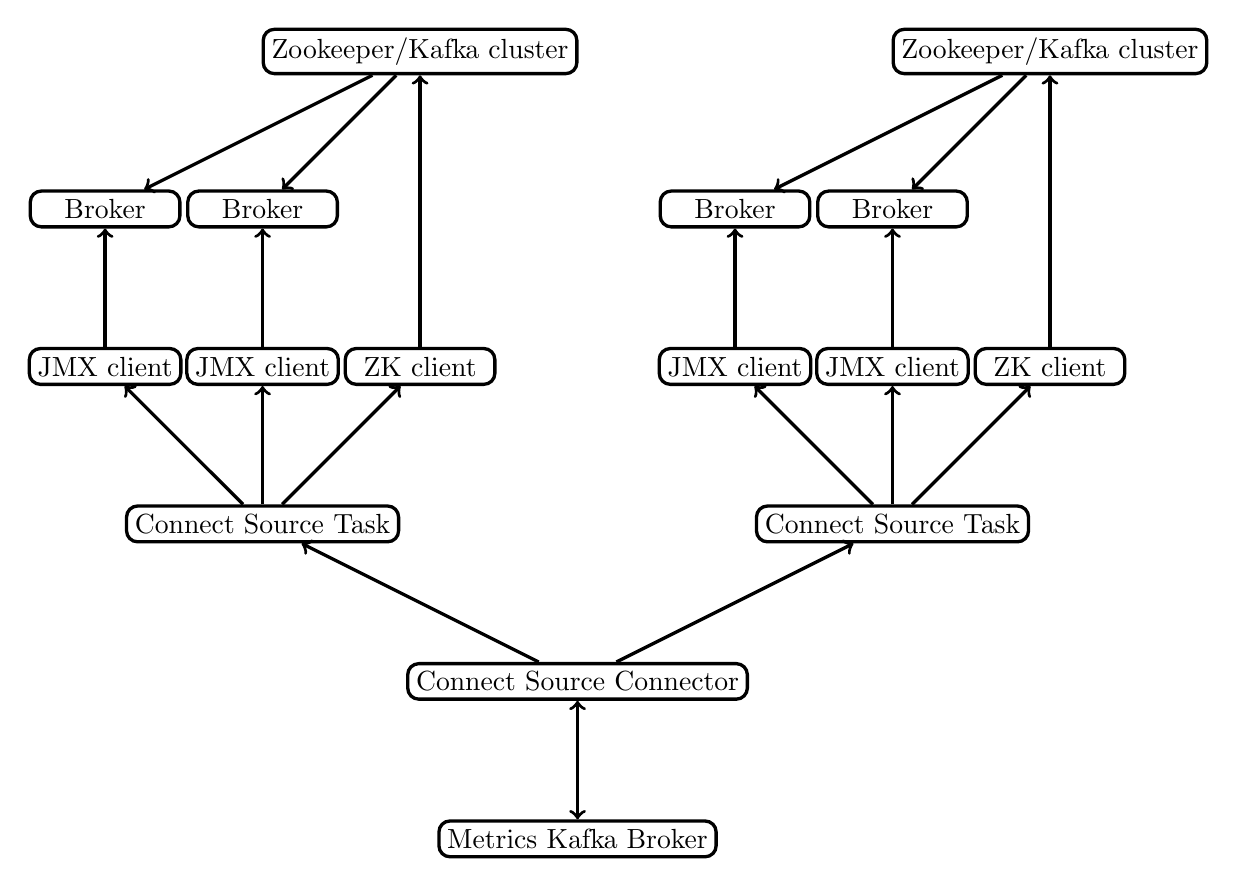
\begin{tikzpicture}[ % has a lot of options; consult the pgf manual
bend angle=45,
square/.style={rectangle, draw=black, fill=white, very thick, inner sep=3pt, minimum width=14mm},
rounded_square/.style={rectangle, rounded corners, draw=black, fill=white, very thick, inner sep=3pt, minimum width=19mm},
both_arrow/.style={<->, very thick},
out_arrow/.style={->, very thick},
in_arrow/.style={<-, very thick},
above_edge_text/.style={above, midway, sloped}
]

% \node[type](name_of_node)[above/below/right/left/...=of name_of_node]{node_text}
%   edge[<->, bend left/right] node[auto, swap]{edge_text}(out_name_of_node)
% OR
% \node[type](name_of_node)[above/below/right/left/...=of name_of_node]{node_text}
\node[rounded_square](zoo_1) at (4,0) {Zookeeper/Kafka cluster};
\node[rounded_square](zoo_2) at (12,0) {Zookeeper/Kafka cluster};

\node[rounded_square](broker_1) at (0,-2) {Broker};
\node[rounded_square](broker_2) at (2,-2) {Broker};
\node[rounded_square](broker_a) at (8,-2) {Broker};
\node[rounded_square](broker_b) at (10,-2) {Broker};

\node[rounded_square](jmx_1) at (0,-4) {JMX client};
\node[rounded_square](jmx_2) at (2,-4) {JMX client};
\node[rounded_square](zk_1) at (4,-4) {ZK client};
\node[rounded_square](jmx_a) at (8,-4) {JMX client};
\node[rounded_square](jmx_b) at (10,-4) {JMX client};
\node[rounded_square](zk_2) at (12,-4) {ZK client};

\node[rounded_square](task_1) at (2,-6) {Connect Source Task};
\node[rounded_square](task_2) at (10,-6) {Connect Source Task};

\node[rounded_square](connector) at (6,-8) {Connect Source Connector};

\node[rounded_square](kafka) at (6,-10) {Metrics Kafka Broker};

% \draw[->](name_of_node.direction) -- (name_of_node.direction)
% OR
% \draw[->](name_of_node.direction) to [bend right] node[]{edge_text} (name_of_node.direction)
% OR
% \draw[->](name_of_node.direction) .. controls +(up/down/right/left:10mm) and +(up/down/right/left:10mm) .. (name_of_node.direction);
\draw[out_arrow](zoo_1) to [] node[auto,swap]{} (broker_1);
\draw[out_arrow](zoo_1) to [] node[auto,swap]{} (broker_2);
\draw[out_arrow](zoo_2) to [] node[auto,swap]{} (broker_a);
\draw[out_arrow](zoo_2) to [] node[auto,swap]{} (broker_b);

\draw[out_arrow](jmx_1) to [] node[auto,swap]{} (broker_1);
\draw[out_arrow](jmx_2) to [] node[auto,swap]{} (broker_2);
\draw[out_arrow](zk_1) to [] node[auto,swap]{} (zoo_1);
\draw[out_arrow](jmx_a) to [] node[auto,swap]{} (broker_a);
\draw[out_arrow](jmx_b) to [] node[auto,swap]{} (broker_b);
\draw[out_arrow](zk_2) to [] node[auto,swap]{} (zoo_2);

\draw[out_arrow](task_1) to [] node[auto,swap]{} (jmx_1);
\draw[out_arrow](task_1) to [] node[auto,swap]{} (jmx_2);
\draw[out_arrow](task_1) to [] node[auto,swap]{} (zk_1);
\draw[out_arrow](task_2) to [] node[auto,swap]{} (jmx_a);
\draw[out_arrow](task_2) to [] node[auto,swap]{} (jmx_b);
\draw[out_arrow](task_2) to [] node[auto,swap]{} (zk_2);

\draw[out_arrow](connector) to [] node[auto,swap]{} (task_1);
\draw[out_arrow](connector) to [] node[auto,swap]{} (task_2);

\draw[both_arrow](kafka) to [] node[auto,swap]{} (connector);
\end{tikzpicture}

\end{document}